\section{Processi primari}

\subsection{Acquisizione}
Il processo di acquisizione comincia con la ricerca e l'identificazione delle necessità espresse dal cliente riguardo il prodotto che vuole ottenere, e tale processo si conclude una volta che queste necessità, opportunamente catalogate e identificate, vengono approvate da quest'ultimo.
L'acquisizione prevede quindi di formulare e catalogare i requisiti, impliciti e non, del progetto in questione.

\subsubsection{Analisi dei requisiti}
\paragraph{Procedura di classificazione requisiti}
Ogni requisito deve essere definito tramite  una descrizione testuale e un codice identificativo, classificante e univoco avente la seguente forma:

\begin{center}\{Tipologia\}\{Importanza\}\{Categoria\}\{Identificatore\}\end{center}


\begin{itemize}

\item Tipologia:
\begin{itemize}
\item \textbf{F:} requisito funzionale;
\item \textbf{Q:} requisito di qualità;
\item \textbf{V:} requisito di vincolo;
\end{itemize}

\item Importanza:
\begin{itemize}
\item \textbf{OB:} requisito obbligatorio;
\item \textbf{DE:} requisito desiderabile;
\item \textbf{OP:} requisito opzionale;
\end{itemize}


\item Categoria:
\begin{itemize}
\item \textbf{U:} requisito funzionale riguardante la parte utente;
\item \textbf{L:} requisito funzionale riguardante la parte utente autenticato;
\item \textbf{A:} requisito funzionale riguardante la parte process owner;
\item vuoto se il requisito è di qualità oppure di vincolo;
\end{itemize}


\item Identificatore è un codice gerarchico composto da uno o più numeri separati da un punto, in cui l'ultimo numero è un identificatore incrementale intero.\\
La rimanente parte di codice viene utilizzata quando il requisito da definire è sotto-requisito di un altro, e identifica il requisito gerarchicamente superiore.

\end{itemize}

\paragraph{Casi d'uso}
Per ciascun caso d'uso deve essere fornito un codice identificativo, una descrizione testuale e un diagramma UML.

\begin{flushleft}
Il codice identificativo deve rispettare la seguente forma:
\end{flushleft}

\begin{center}UC\{Tipologia\}\{Identificatore\}\end{center}
Tipologia può essere U, L o A, che stanno rispettivamente per utente non autenticato, utente autenticato e process owner.\\
Identificatore è un codice gerarchico composto da uno o più numeri separati da un punto, in cui l'ultimo numero è un identificatore incrementale intero.
La rimanente parte di codice viene utilizzata quando il caso d'uso da definire è una specifica o estensione di un altro, e identifica il caso d'uso gerarchicamente superiore.

\begin{flushleft}
La descrizione deve contenere i seguenti dettagli:
\end{flushleft}

\begin{itemize}
\item Descrizione del caso d'uso;
\item Attori coinvolti;
\item Precondizione;
\item Scenario principale dello svolgersi degli eventi;
\item Senari alternativi;
\item Post-condizione.
\end{itemize}

\begin{flushleft}
Il diagramma deve rispettare le regole della notazione UML 2.x\ped{G}.
\end{flushleft}
\paragraph{Strumenti per l'analisi}
\subparagraph{Piattaforma per il tracciamento}
Per il tracciamento è stato sviluppato un semplice programma denominato \textit{Sirius RTg}. Questo programma è stato sviluppato utilizzando PHP\ped{G}, CSS\ped{G} ed HTML\ped{G}. Sirius RTg è attualmente un programma il cui sviluppo non è terminato, principalmente per permettere una aggiunta di funzionalità in caso di necessità. Sirius RTg, alla versione 2.0.0, fornisce le seguenti funzionalità:
\begin{itemize}
\item Inserimento requisito e relativo tracciamento;
\item Visualizzazione dello script per la tabella dei requisiti e relativo tracciamento.
\end{itemize}
\subparagraph{Inserimento requisito e relativo tracciamento}
Questa funzionalità è fornita all'esterno attraverso un'interfaccia scritta in HTML e CSS.\\
L'interfaccia è costituita da uno semplice \textit{form}, in cui è possibile inserire:
\begin{itemize}
\item Codice requisito;
\item Descrizione del requisito;
\item Categoria;
\item Importanza;
\item Tipo;
\item Relativi casi d'uso;
\item Relative fonti.
\end{itemize}
Ogni requisito deve avere obbligatoriamente definito il Tipo, l'Importanza, ed il Codice requisito. Il codice deve necessariamente identificare univocamente il requisito, altrimenti un uso ridondante di codici verrà notificato all'utente. Obbligatoria la categoria, in caso il requisiti sia della parte utente.
\subparagraph{Visualizza script}
Questa funzionalità serve per la stampa a video dei vari script in \LaTeX{} per i vari requisiti e il relativo tracciamento.\\ Visualizza script è composto dalle seguenti funzionalità:
	\begin{itemize}
		\item Visualizzazione script per Requisiti di tipo utente amministratore;
		\item Visualizzazione script per Requisiti di tipo utente-utente autenticato;
		\item Visualizzazione script per Requisiti di vincolo;
		\item Visualizzazione script per Requisiti di qualità;
		\item Visualizzazione script tracciamento Requisiti-uc;
		\item Visualizzazione script tracciamento Uc-requisiti.
	\end{itemize}
Ogni script stampato su video, segue le regole definite nelle \textit{Norme di Progetto}.\\
Anche se Visualizzazione script utente e Visualizzazione script utente autenticato sono due sotto-funzionalità distinte di Visualizza script, devono essere utilizzate assieme per produrre la tabella dei requisiti di tipo utente; infatti Visualizzazione script utente stampa l'intestazione della tabella e la parte dei requisiti utente, mentre Visualizzazione script utente autenticato stampa la parte dei requisiti utente autenticato e i comandi necessari per chiudere la tabella.\\
Tutti gli altri Script, invece possono essere usati singolarmente e a video, oltre al contenuto comparirà la relativa intestazione e chiusura della tabella.
\subparagraph{Inserimento componente e relativo tracciamento}
Questa funzionalità è stata inserita al fine di poter tracciare le componenti del sistema, permette di inserire tramite un form:
\begin{itemize}
\item Nome del componente
\item Requisiti associati al componente
\end{itemize}
Sono state inoltre implementati due script che stampano a video il codice \LaTeX{} del tracciamento componente-requisito e requisito-componente, il codice \LaTeX{} generato è conforme alle \NormeDiProgetto{}.
\subparagraph{Script glossario}
Anche se non inerente al tracciamento dei requisiti, lo strumento \textit{Sirius RTg} alla versione 2.0 prevede la funzionalità aggiuntiva di poter inserire automaticamente i pedici \ped{G} (per le parole contenute nel \Glossario{}) ai documenti del team.
\subsection{Fornitura}
Il processo di fornitura agglomera le attività di: gestione delle pianificazione, gestione delle risorse, gestione dei rischi.
Tale processo quindi ha come obbiettivo quello di fornire un\textbf{ piano} per la gestione del progetto che imponga delle direttive in merito alla:
\begin{itemize}
\item pianificazione delle attività;
\item pianificazione delle milestone;
\item pianificazione delle scadenze.
\end{itemize}
Il responsabile di tutto questo, durante il corso dell'intero progetto, è il \textit{Responsabile di progetto}.


\subsubsection{Pianificazione}
Il \textit{responsabile di progetto} per ogni attività indicata nel documento \textit{Piano di Progetto} dovrà creare un nuovo progetto seguendo la procedura qui descritta:

\begin{enumerate}
\item Inserire una milestone\ped{G};
\item Inserire le attività da svolgere;
\item Inserire le rispettive sotto-attività;
\item Calcolare ed inserire i periodi di slack\ped{G} qualora fosse necessario;
\item Creare le risorse;
\item Assegnare le risorse create ad ogni attività;
\item Salvare la baseline\ped{G}.
\end{enumerate}

Sarà decisa a discrezione del \textit{Responsabile di Progetto} per ogni attività la possibilità di assegnare un surplus di ore, queste ore supplementari verranno scelte basandosi sulla criticità dell'attività considerata. 
\begin{itemize}
\item Per le attività non critiche non è previsto alcun surplus di ore;
\item Per le attività di media criticità il surplus di ore potrà essere del 15\%;
\item Per le attività di criticità massima il surplus di ore potrà essere del 30\%.
\end{itemize}
\paragraph{Procedura utilizzo del ticketing}
Ogni membro del team \textit{Sirius} avrà accesso al sistema di \textit{ticketing}. Le figure che invece potranno assegnare ticket sono le seguenti:

\begin{itemize}
\item Il \textit{Responsabile di Progetto} assegnerà i \textit{ticket} di massima importanza cioè quelli correlati allo sviluppo delle attività necessarie all' avanzamento del progetto;
\item Il \textit{Verificatore} potrà assegnare \textit{ticket} allo scopo di segnalare errori di grave entità rilevati durante l'attività di verifica.
\end{itemize}

Di conseguenza i \textit{ticket} sono suddivisi in due macro-categorie:
\begin{itemize}
\item \textit{Ticket} di pianificazione, i quali rappresentano le attività che devono essere svolte per procedere con l'avanzamento del progetto, sono suddivisi in 4 sotto-categorie:
\begin{itemize}
\item \emph{Documento}: che rappresenta una \textit{task} inerente alla redazione di un documento; 
\item \emph{Codice}: che rappresenta una \textit{task} inerente alla stesura di codice;
\item \emph{Verifica}: che rappresenta una \textit{task} inerente all'attività di verifica di un'attività;
\item \emph{Generali}: che rappresenta \textit{tasks} i cui scopi sono svariati ed in genere non ad alta priorità, come ad esempio la ricerca di un determinato \textit{software}.
\end{itemize}
lo svolgimento dell'insieme di tutti i ticket di una \textit{task-list} non porterà alla conclusione della \textit{task-list} stessa, questo poiché è prevista la possibilità di aggiungere durante l'avanzamento del progetto ulteriori \textit{task}, fino a quando il \textit{responsabile di progetto} non ne dichiarerà la conclusione;
\item Ticket di verifica, contenenti gli errori identificati dai \textit{verificatori} a seguito dell'analisi del lavoro svolto da qualche membro del \textit{team}.
\end{itemize}

Ogni membro del \textit{team} sarà tenuto ad utilizzare la barra di avanzamento di stato del \textit{ticket} fornita dall'interfaccia di \textit{TeamWorkPM}, evitando così superflue norme aggiuntive atte a determinare lo stato del \textit{ticket}.

\paragraph{Procedura creazione di una milestone}
Il \textit{Responsabile di Progetto} dovrà creare una \textit{milestone}, essa indica la data della revisione a cui il gruppo \gruppo{} intende presentarsi, è possibile visualizzare lo stato di avanzamento che tiene conto del numero di \textit{ticket} completati rispetto al numero di \textit{ticket} complessivi.
Per la creazione di una nuova \textit{milestone} il \textit{Responsabile di Progetto} dovrà seguire i seguenti passi:
\begin{enumerate}
\item Aprire il progetto dall'interfaccia \textit{web} di \textit{TeamWorkPM};
\item Posizionarsi sull'opzione: "\emph{Milestones}" ed accedervi;
\item Cliccare sull'opzione: "\emph{Add a new milestone}".
\end{enumerate}

Completati questi passaggi apparirà il seguente \textit{form\ped{G}} (fig 1) che dovrà essere compilato per concludere la creazione della una \textit{milestone}.
\begin{figure}
\centering
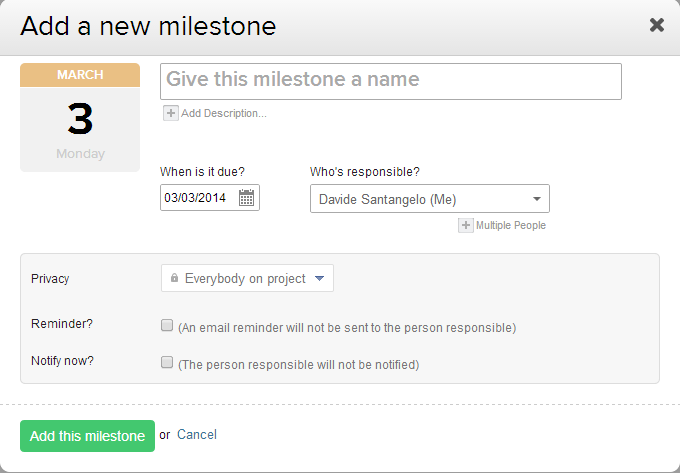
\includegraphics[width=%
\textwidth]{immaginiNDP/Immagine}
\caption[]{Creazione di una milestone.}
\label{fig:Immagine}
\end{figure}

\paragraph{Procedura di creazione ticket} 
Il \textit{Responsabile di Progetto} dovrà attenersi alla seguente procedura per la creazione di una nuova task-list, ovvero la concretizzazione di un macro-attività e delle sue relative task (ticket). Si ricorda che TeamWorkPM prevede la possibilità di indicare interdipendenze tra task-list.
\begin{enumerate}
\item Dall'interfaccia \textit{web} accedere al progetto \progetto{}, e selezionare dal \textit{menù} principale il comando: \emph{"Task"};
\item Procedere, se necessario, con la creazione di una nuova \textit{task-list} tramite il comando: \emph{"Add task list"};
\item Una volta creata la \textit{task-list} sarà possibile creare i \textit{ticket} (\textit{Task} nel contesto di \textit{TeamWorkPM}) inerenti alla \textit{task-list} scelta.
\end{enumerate}

La struttura di un \textit{ticket} è visualizzabile nella figura 2 di questa sezione.
\begin{figure}
\centering
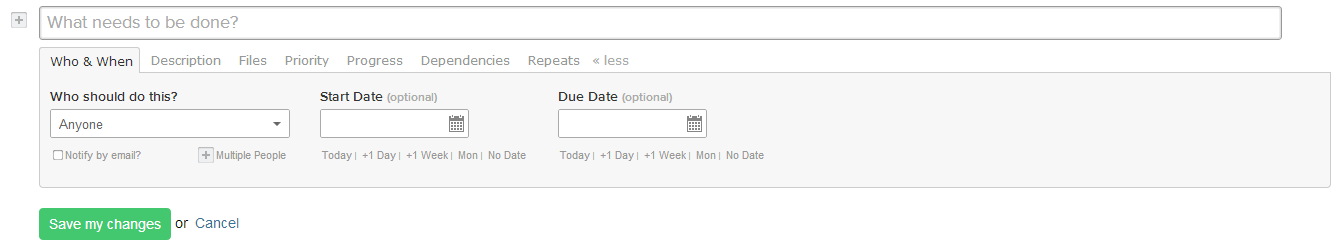
\includegraphics[width=%
\linewidth]{immaginiNDP/creazionetask}
\caption[]{Creazione di un ticket.}
\label{fig:creazionetask}
\end{figure}

Nella task è necessario specificare \textbf{obbligatoriamente}:
\begin{itemize}
\item Il \textbf{Titolo} del \textit{ticket}, dovrà contenere tra parentesi quadre la categoria (per i \textit{ticket} di pianificazione anche la sotto-categoria) di \textit{ticket} di cui si tratta;
\item Il \textbf{Destinatario} del \textit{ticket}, cioè colui a cui è stato assegnato;
\item Le \textbf{Date} di inizio e scadenza del \textit{ticket};
\item Le \textbf{Dipendenze} del \textit{ticket}, che specificano l' eventuale necessità di attendere la terminazione di un insieme di \textit{task} prima di poter svolgere quel determinato compito;
\item Una \textbf{Descrizione} la quale dovrà essere breve e coincisa, ma spiegare efficacemente il lavoro assegnato;
\item La \textbf{Priorità} del \textit{ticket} suddivisa in tre categorie: bassa, media, alta.
\end{itemize}

Compilati i seguenti campi, il \textit{ticket} sarà creato ed inviato regolamentarmene.

\paragraph{Procedura di terminazione ticket}
Se un \textit{ticket} sarà completato è necessario applicare questa procedura di accertamento:
\begin{enumerate}
\item Il membro del \textit{team} a cui è stato assegnato il \textit{ticket} dovrà spuntare la casella di terminazione su \textit{TeamWorkPM};
\item Durante il controllo giornaliero il \textit{Responsabile di Progetto} controllerà quanto necessario a determinare che il lavoro sia stato effettivamente svolto;
\item Se il lavoro è stato effettivamente svolto, sarà avviato un \textit{ticket} di \emph{Pianificazione} a scopo di verificare il lavoro;
\item Nel caso di irregolare svolgimento del \textit{ticket} o problemi di grave entità, il \textit{Responsabile di Progetto} dovrà applicare la procedura di modifica o riassegnazione del \textit{ticket} presente nel prossimo paragrafo;
\item Nel caso di esito positivo (cioè con regolare svolgimento) il \textit{ticket} sarà concluso ed archiviato, mentre al contempo, qualora fosse necessario, saranno avviati dei \textit{ticket} di \emph{Verifica} per la correzione degli errori non gravi rilevati durante la \textit{Verifica};

\end{enumerate}

\paragraph{Procedura per la modifica o riassegnazione ticket} 
Durante il suo ciclo di vita un \textit{ticket} per varie ragioni può andare in contro a modifiche, è necessario quindi normare la seguente procedura:
\begin{enumerate}
\item Aprire il progetto dall'interfaccia \textit{web} di \textit{TeamWorkPM};
\item Selezionare il \textit{ticket} di interesse;
\item Selezionare il comando: \emph{"Edit Task"};
\item Aggiungere una descrizione riguardo la modifica effettuata;
\item Avvertire l'interessato che è stata effettuata una modifica inserendo: "(MOD)" sul titolo del \textit{ticket}, e qualora fosse necessario reimpostandone la sua priorità.
\end{enumerate}
\paragraph{Strumento per la gestione del progetto}
Al fine di gestire rigorosamente lo sviluppo del progetto il team \gruppo{} ha adottato l'utilizzo del software \textit{TeamWorkPM} (\href{http://www.teamwork.com}{www.teamwork.com}), tale strumento fornisce le seguenti funzionalità:

\begin{itemize}
\item Creazione di \textit{ticket\ped{G}}, \textit{milestone\ped{G}} e liste di attività;
\item Creazione ed assegnazione di attività;
\item Calendario di progetto;
\item \textit{Report} automatico giornaliero delle attività svolte ed in ritardo inviato tramite \textit{e-mail};
\item Gestione dei ruoli;
\item Generazione di grafici \textit{Gantt\ped{G}} a partire dalle \textit{task-list};
\item Monitoraggio dei tempi;
\item Registro dei rischi.
\end{itemize}

Sono stati valutati altri software come ad esempio \textit{Redmine}, il quale fu ritenuto quasi altrettanto completo ed intuitivo. Tuttavia si è optato per \textit{TeamWorkPM} data la sua estrema semplicità di utilizzo.\\
Il \textit{Responsabile di Progetto} per garantire il regolare svolgimento delle attività dovrà necessariamente verificare con cadenza giornaliera se sono presenti \textit{ticket} scaduti e non ancora completati, nel caso citato infatti sarà obbligato a richiedere informazioni (o in caso di ritardi gravi convocare l'interessato) circa la causa del ritardo.\\
Infine, il \textit{Responsabile di Progetto} dovrà tenere nota che l'assegnazione di \textit{ticket} la cui scadenza è prevista per il giorno successivo può avvenire solo se il lavoro da svolgere non supera le 2 ore lavorative.


\paragraph{Strumenti per la pianificazione}
\subparagraph{GanttProject}
Per la pianificazione del progetto nonché gestione delle risorse è stato adottato il software GanttProject, software open source basato su piattaforma Java. Qui di seguito vengono elencate le principali caratteristiche che hanno portato alla scelta di questo strumento:
\begin{itemize}
\item Portabilità, essendo un software basato su Java;
\item Open-source\ped{G};
\item Compatibile con MicrosoftProject;
\item Può generare grafici Work Breakdown Structure (WBS\ped{G});
\item Fornisce la possibilità di creare grafici di Gantt\ped{G};
\item Può generare grafici Program Evalutation and Review Tecnique (PERT\ped{G});
\item In grado di gestire e generare grafici delle risorse assegnate.
\end{itemize}

\subparagraph{Team Work PM}
Al fine di gestire rigorosamente lo sviluppo del progetto il team \gruppo{} ha adottato l'utilizzo del software \textit{TeamWorkPM} (\href{http://www.teamwork.com}{www.teamwork.com}), tale strumento fornisce le seguenti funzionalità:

\begin{itemize}
\item Creazione di \textit{ticket\ped{G}}, \textit{milestone\ped{G}} e liste di attività;
\item Creazione ed assegnazione di attività;
\item Calendario di progetto;
\item \textit{Report} automatico giornaliero delle attività svolte ed in ritardo inviato tramite \textit{e-mail};
\item Gestione dei ruoli;
\item Generazione di grafici \textit{Gantt\ped{G}} a partire dalle \textit{task-list};
\item Monitoraggio dei tempi;
\item Registro dei rischi.
\end{itemize}

Sono stati valutati altri software come ad esempio \textit{Redmine}, il quale fu ritenuto quasi altrettanto completo ed intuitivo. Tuttavia si è optato per \textit{TeamWorkPM} data la sua estrema semplicità di utilizzo.\\
Il \textit{Responsabile di Progetto} per garantire il regolare svolgimento delle attività dovrà necessariamente verificare con cadenza giornaliera se sono presenti \textit{ticket} scaduti e non ancora completati, nel caso citato infatti sarà obbligato a richiedere informazioni (o in caso di ritardi gravi convocare l'interessato) circa la causa del ritardo.\\
Infine, il \textit{Responsabile di Progetto} dovrà tenere nota che l'assegnazione di \textit{ticket} la cui scadenza è prevista per il giorno successivo può avvenire solo se il lavoro da svolgere non supera le 2 ore lavorative.
\subsection{Sviluppo}
\subsubsection{Progettazione}
Questa sezione descrive le norme cui i progettisti dovranno attenersi durante la stesura del documento:  \textit{Specifica tecnica} ed il documento \textbf{definizione di prodotto}. Queste norme sono dettate al fine di poter redigere un documento il più possibile formale e senza ambiguità.

\subsubsection{Specifica tecnica}
\paragraph{Diagrammi}
Per quanto concerne i diagrammi sarà adottato il linguaggio \textit{Unified Modelling Language}(UML) 2.0,
tramite questo linguaggio si andranno a definire:
\begin{itemize}
\item \textbf{Diagrammi dei package}: ossia elementi di raggruppamento di classi. Tali elementi dovranno figurare durante la progettazione generale e dovranno essere identificati univocamente al fine di stabilire come i suddetti interagiscono tra di loro.

\item \textbf{Diagrammi di sequenza}: I quali andranno a descrivere come un gruppo di oggetti andranno a collaborare per implementare collettivamente un comportamento;

\item \textbf{Diagrammi di attività}: Atti a mostrare i flussi di attivit che gli utenti potranno percorrere durante l'uso dell'applicazione;

\item \textbf{Diagrammi delle classi}: I quali consentono di descrivere tipi di entità con le loro caratteristiche.
\end{itemize}

\paragraph{Design pattern}
Per ogni design pattern utilizzato sarà necessario andare a definire i seguenti punti:
\begin{itemize}
\item Una \textbf{descrizione generale} che riporta la struttura del design pattern scelto;
\item Una \textbf{motivazione} che descriva i vantaggi che ne comporta il suo uso;
\item Il \textbf{contesto applicativo} che associa ai design pattern utilizzati il contesto dove sono stati adottati.
\end{itemize}

\paragraph{Nomenclatura delle classi}
Ogni classe descritta nel documento specifica tecnica seguirà il seguente schema:
\begin{itemize}
\item \textbf{Nome}: enuncia il nome della classe che andrà descritta, devono essere obbligatoriamente in inglese e devono comparire con l'iniziale in maiuscolo.
\item \textbf{Package}:enuncia il pacchetto, ed i relativi sotto-pacchetti, all'interno dei quali è contenuta la classe di interesse.
Ogni package deve seguire la seguente notazione: Pack1::Pack2::..::Pack-n;
ove con:
\begin{itemize}
\item Pack1, si intende il package principale;
\item Pack(x)::Pack(y) indica che indica che y è sotto package di x;
\end{itemize}

\item \textbf{Descrizione}: deve contenere una breve ma significativa descrizione testuale riguardante l'utilizzo della classe;
\item \textbf{Relazione con altri componenti}: viene specificato se la classe di interesse ha relazioni con le classi di altri componenti.
\end{itemize}

\paragraph{Tracciamento}
Ogni componente sarà tracciato seguendo tali regole:\\
\begin{center}
{\textbf{Ambito}}{\textbf{Utente}}{\textbf{Codice}}
\end{center}

ove \textbf{Ambito} rappresenta con:
\begin{itemize}
\item \textbf{V}: view;
\item \textbf{CP}: client presenter;
\item \textbf{SP}: server presenter;
\item \textbf{CM}: client model;
\item \textbf{SM}: server model.
\end{itemize}

ove \textbf{Ambito} rappresenta:
\begin{itemize}
\item \textbf{A}: process owner;
\item \textbf{U}: utente;
\end{itemize}

Per quanto concerne il codice, si adotteranno i codici del tracciamento degli UC.

\paragraph{Test} I progettisti avranno il compito di definire delle classi e dei test fittizi con lo scopo di valutare il lavoro svolto.
I test saranno suddivisi in:
\begin{itemize}
\item Test di integrazione;
\item Test di unità;
\end{itemize}

\paragraph{Tracciamento requisiti-componenti}

\begin{itemize}
\item \textit{Requisito}: contiene il codice univoco e classificante del requisito;
\item \textit{Descrizione requisito}: contiene la descrizione del requisito;
\item \textit{Nome componente}: contiene il codice identificativo del componente.
\end{itemize}

\paragraph{Tracciamento componenti-requisiti}
La struttura della tabella sarà la seguente:
\begin{itemize}
\item \textit{Requisito}: contenente il codice univoco e classificante del requisito;
\item \textit{Componente}: contente il nome del package ed il nome della classe.
\end{itemize}

\paragraph{Test di sistema ed integrazione}
Il tracciamento dei test sarà inserito in forma tabellare nel documento \PianoDiQualifica, e dovrà rispettare il seguente stampo:
\begin{itemize}
\item \textbf{Codice test}: il quale dovrà essere obbligatoriamente univoco ed atto ad identificare il test;
\item \textbf{Descrizione}: la quale specifica lo scopo del test;
\item \textbf{Requisito annesso}: che specifica il requisito cui il test fa riferimento;
\item \textbf{Stato}: che riporta se il test è stato effettuato.
\end{itemize}

\subsubsection{Definizione di prodotto}
Redigere il documento di \textit{definizione di prodotto} sarà compito dei \textit{progettisti}.
La \textit{definizione di prodotto} è un documento che si pone l'obbiettivo di definire dettagliatamente ogni singola unità di cui è composto il sistema. Al fine di non lasciare libertà di iniziativa durante l'attività di codifica sarà necessario quindi specificare i metodi e gli  attributi di ogni classe.
Questo documento presenterà una versione più raffinata, rispetto alla specifica tecnica, dei seguenti diagrammi:
\begin{itemize}
\item \textbf{Diagrammi delle classi};
\item \textbf{Diagrammi di sequenza}.
\end{itemize}
\paragraph{Formalismo delle classi}
Ogni classe deve essere definita attenendosi alle seguenti convenzioni:
\begin{itemize}
\item \textbf{attributi:} dovranno essere indicati specificando il grado di accessibilità come previsto da UML 2.4. Infine dovrà seguire (riportata sotto il diagramma) la descrizione dell’attributo stesso.
\item \textbf{metodi:}come per gli attributi si dovrà specificare il grado di accessibilità dei
suddetti, a seguito dovrà figurare il nome del metodo stesso. Tra parentesi tonde si
dovranno inserire i suoi parametri. Infine si inserirà il tipo di ritorno del metodo.
\item \textbf{parametri:} i parametri, racchiusi da parentesi tonde, devono presentare il loro nome seguito da due punti ed il loro tipo.
\end{itemize}
\subsubsection{Norme sulla codifica}
\paragraph{Convenzioni di codifica}
Al fine di produrre codice ordinato e leggibile, in modo da semplificare il più possibile l'attività di manutenzione, per quanto concerne la programmazione \textit{Java\ped{G}}, si adotteranno le norme imposte dalla \textit{Java code conventions}, reperibili all'indirizzo:
\begin{center}
\href{http://www.oracle.com/technetwork/java/codeconvtoc-136057.html}{http://www.oracle.com/technetwork/java/codeconvtoc-136057.html}
\end{center}
Variazioni e modifiche a queste convenzioni possono essere richieste all'\textit{Amministratore}, allegandone la motivazione.
Se l'\textit{Amministratore} riterrà opportune le variazioni presentate, sarà tenuto a notificarlo al team seguendo le convenzioni imposte dalle \textit{Norme di Progetto}.

\paragraph{Nomi}
Sarà adottata la notazione \textit{CamelCase} al fine di identificare facilmente il nome di variabili, classi, metodi, funzioni, interfacce. Più specificatamente bisognerà rispettare le seguenti regole:
\begin{itemize}
\item \textbf{variabili, metodi, funzioni, interfacce}:dovranno avere la prima lettera minuscola;
\item \textbf{classi}: dovranno avere la prima lettera maiuscola.
\end{itemize}
Inoltre sarà obligatorio utitilizzare la lingua \textbf{inglese} per assegnare i suddetti nomi. 
Inoltre è opportuno ma non obbligatorio che i nomi (di variabili, metodi, etc..) siano esplicativi rispetto al ruolo che assumono nel contesto di applicazione.

\paragraph{Commenti ed intestazioni}

Ogni file contenente codice dovrà essere provvisto di un intestazione che rispetta la seguente forma:
\\
\\
\textcolor{green}{
\textbf{file}: che riporta il nome del file; \\
\textbf{author}: che riporta il nome dell'autore;\\
\textbf{date}: che riporta la data di creazione; \\
\textbf{lastModified}: che riporta la data di ultima modifica;\\
\textbf{brief}: che descrive brevemente lo scopo e contenuto del file.\\
}

Le classi dovranno obbligatoriamente essere provviste di commenti che contengono:
\\
\\
\textcolor{green}{
\textbf{class}: nome della classe;\\
\textbf{brief}: breve descrizione della classe.\\
}
Per quanto concerne i metodi, essi dovranno essere provvisti di commenti che si adeguano alla seguente forma:
\\
\\
\textcolor{green}{
\textbf{brief}: breve descrizione del compito del metodo;\\
\textbf{param}: che comparirà tante volte quanti sono i parametri in input al metodo, e ne riporterà il nome ed il tipo;\\
\textbf{return}: nome e tipo del valore ritornato dalla funzione.\\}

Infine per le interfacce la forma sarà la seguente:
\\
\\
\textcolor{green}{
\textbf{brief}: breve descrizione dello scopo dell'interfaccia.\\}

Qualora fosse impossibile utilizzare la tecnica del \textit{refractoring}\ped{G} per ristrutturare il codice, nel qualcaso si trattasse di codice particolarmente difficile da comprendere, è possibile dedicare un commento aggiuntivo:
\\
\\
\textcolor{green}{spiegazione approfondita: ...\\}\\
al fine di facilitarne la comprensione.
\paragraph{Strumenti per la codifica}
Il team \gruppo{} durante lo sviluppo dell'applicazione utilizzerà diversi framework e librerie quali:

\begin{itemize}
\item Spring;
\item Backbone.js;
\item RequireJS.
\end{itemize}

Per non incorrere in problemi di incompatibilità del codice sviluppato, si è deciso di uniformare le versioni di tali \textit{framework} e librerie.
I programmatori sono quindi \textbf{tenuti} a sviluppare tramite software aggiornato alla seguente \textit{release}:
\begin{itemize}
\item \textbf{\textit{Spring:}} 4.0.3;
\item \textbf{\textit{Backbone.js:}} 1.1.2;
\item \textbf{\textit{RequireJS:}} 1.1.
\end{itemize}





\paragraph{IDE}
Per la stesura del codice dell'applicazione \progetto{} il team \gruppo{} sara tenuto ad utlizzare gli ide\ped{G} ammessi nella lista di seguito riportata. Nel caso il team di sviluppo lo ritenesse necessario, sarà possibile richiedere all'\textit{amministratore} di modificare tale lista aggiungendo nuovi ambienti di sviluppo che vengono ritenuti più adatti per la stesura del codice.
\\
\\
\textbf{Spring tool suite (versione 3.5.1)}.
\\
\\
\textit{Spring tool suite} è un ide basato su Eclipse che integra tutto il necessario per lavorare ad un progetto che necessita l'utilizzo del \textit{framework} \textit{Spring}.
\\
\\
Infine è possibile utilizzare l'ide \textit{Eclipse} in quanto si tratta di un ambiente di sviluppo \textit{open source} multipiattaforma e multilinguaggio piuttosto completo, con possibilità di installare plug-in per espanderne le sue funzionalità.
La versione da adottare di questo software è la 4.3.2 (Kepler SR2).


